The results are presented in four steps. Section~\ref{sec:resA} reports
the performance of the HS models under the resample-before-split protocol
(Protocol A). Section~\ref{sec:leak} analyses why these results do not
transfer to new patients. Section~\ref{sec:resB} evaluates the same models
and the improved pipeline on real, held-out records (Protocol B), including
an ablation study and five-fold cross-validation, and
Section~\ref{sec:compare} compares the findings with existing studies. All
experiments use a fixed random state of 42 and can be reproduced with the
released code.

\subsection{Performance under the Resample-Before-Split Protocol}
\label{sec:resA}

Table~\ref{tab:protoA} reports the test-set performance of all models when
the full dataset is resampled before it is split (Protocol A), as in the
original pipeline. With hybrid sampling every model appears highly
accurate: the DT reaches 99.78\% accuracy and 100\% recall, XGBoost
98.23\%, the MLP 98.45\% and the CNN and NN 96.02\% and 94.70\%; the ROC
curves (Fig.~\ref{fig:rocA}) hug the top-left corner with AUC values of
0.96--1.00. Models trained with ROS alone, in contrast, reach only about
75.5\% accuracy and an AUC of 0.83. The last column lists the accuracies
reported in the original version of this study; our reimplementation
reproduces them closely for HS and ROS. For SMOTEENN alone our
reimplementation obtains higher values than originally reported (88.6--91.2\%
vs.\ 74--75\%), consistent with the effect of ENN cleaning on the test set
discussed in Section~\ref{sec:leak}.

\begin{table}[t]
\centering
\caption{Test performance under Protocol A (resample before split; 3,000
test records per class drawn from the resampled data). Last column:
accuracy reported in the original version of this study.}
\label{tab:protoA}
\small
\begin{tabular}{llcccccc}
\toprule
Sampling & Model & Acc. (\%) & Prec. (\%) & Rec. (\%) & F1 (\%) & AUC (\%) & Orig. Acc. (\%) \\
\midrule
\multirow{3}{*}{SMOTEENN} & CNN & 88.58 & 96.81 & 79.80 & 87.48 & 98.08 & 74.09 \\
 & NN & 89.18 & 96.41 & 81.40 & 88.27 & 98.38 & 75.08 \\
 & MLP & 91.15 & 97.72 & 84.27 & 90.50 & 99.12 & 75.00 \\
\midrule
\multirow{3}{*}{ROS} & CNN & 75.55 & 72.70 & 81.83 & 77.00 & 83.17 & 75.13 \\
 & NN & 75.47 & 72.63 & 81.73 & 76.91 & 83.20 & 75.51 \\
 & MLP & 75.63 & 72.39 & 82.87 & 77.28 & 83.30 & 75.91 \\
\midrule
\multirow{6}{*}{HS} & CNN & 96.02 & 93.13 & 99.37 & 96.15 & 98.73 & 93.01 \\
 & NN & 94.70 & 94.49 & 94.93 & 94.71 & 98.63 & 95.96 \\
 & MLP & 98.45 & 97.12 & 99.87 & 98.47 & 99.47 & 97.55 \\
 & DT & 99.78 & 99.57 & 100.00 & 99.78 & 99.78 & 99.70 \\
 & SVM & 89.57 & 88.79 & 90.57 & 89.67 & 95.96 & 93.16 \\
 & XGBoost & 98.23 & 96.80 & 99.77 & 98.26 & 99.65 & 97.80 \\
\bottomrule
\end{tabular}
\end{table}

\begin{figure}[t]
\centering
\begin{subfigure}{0.49\linewidth}
  \centering
  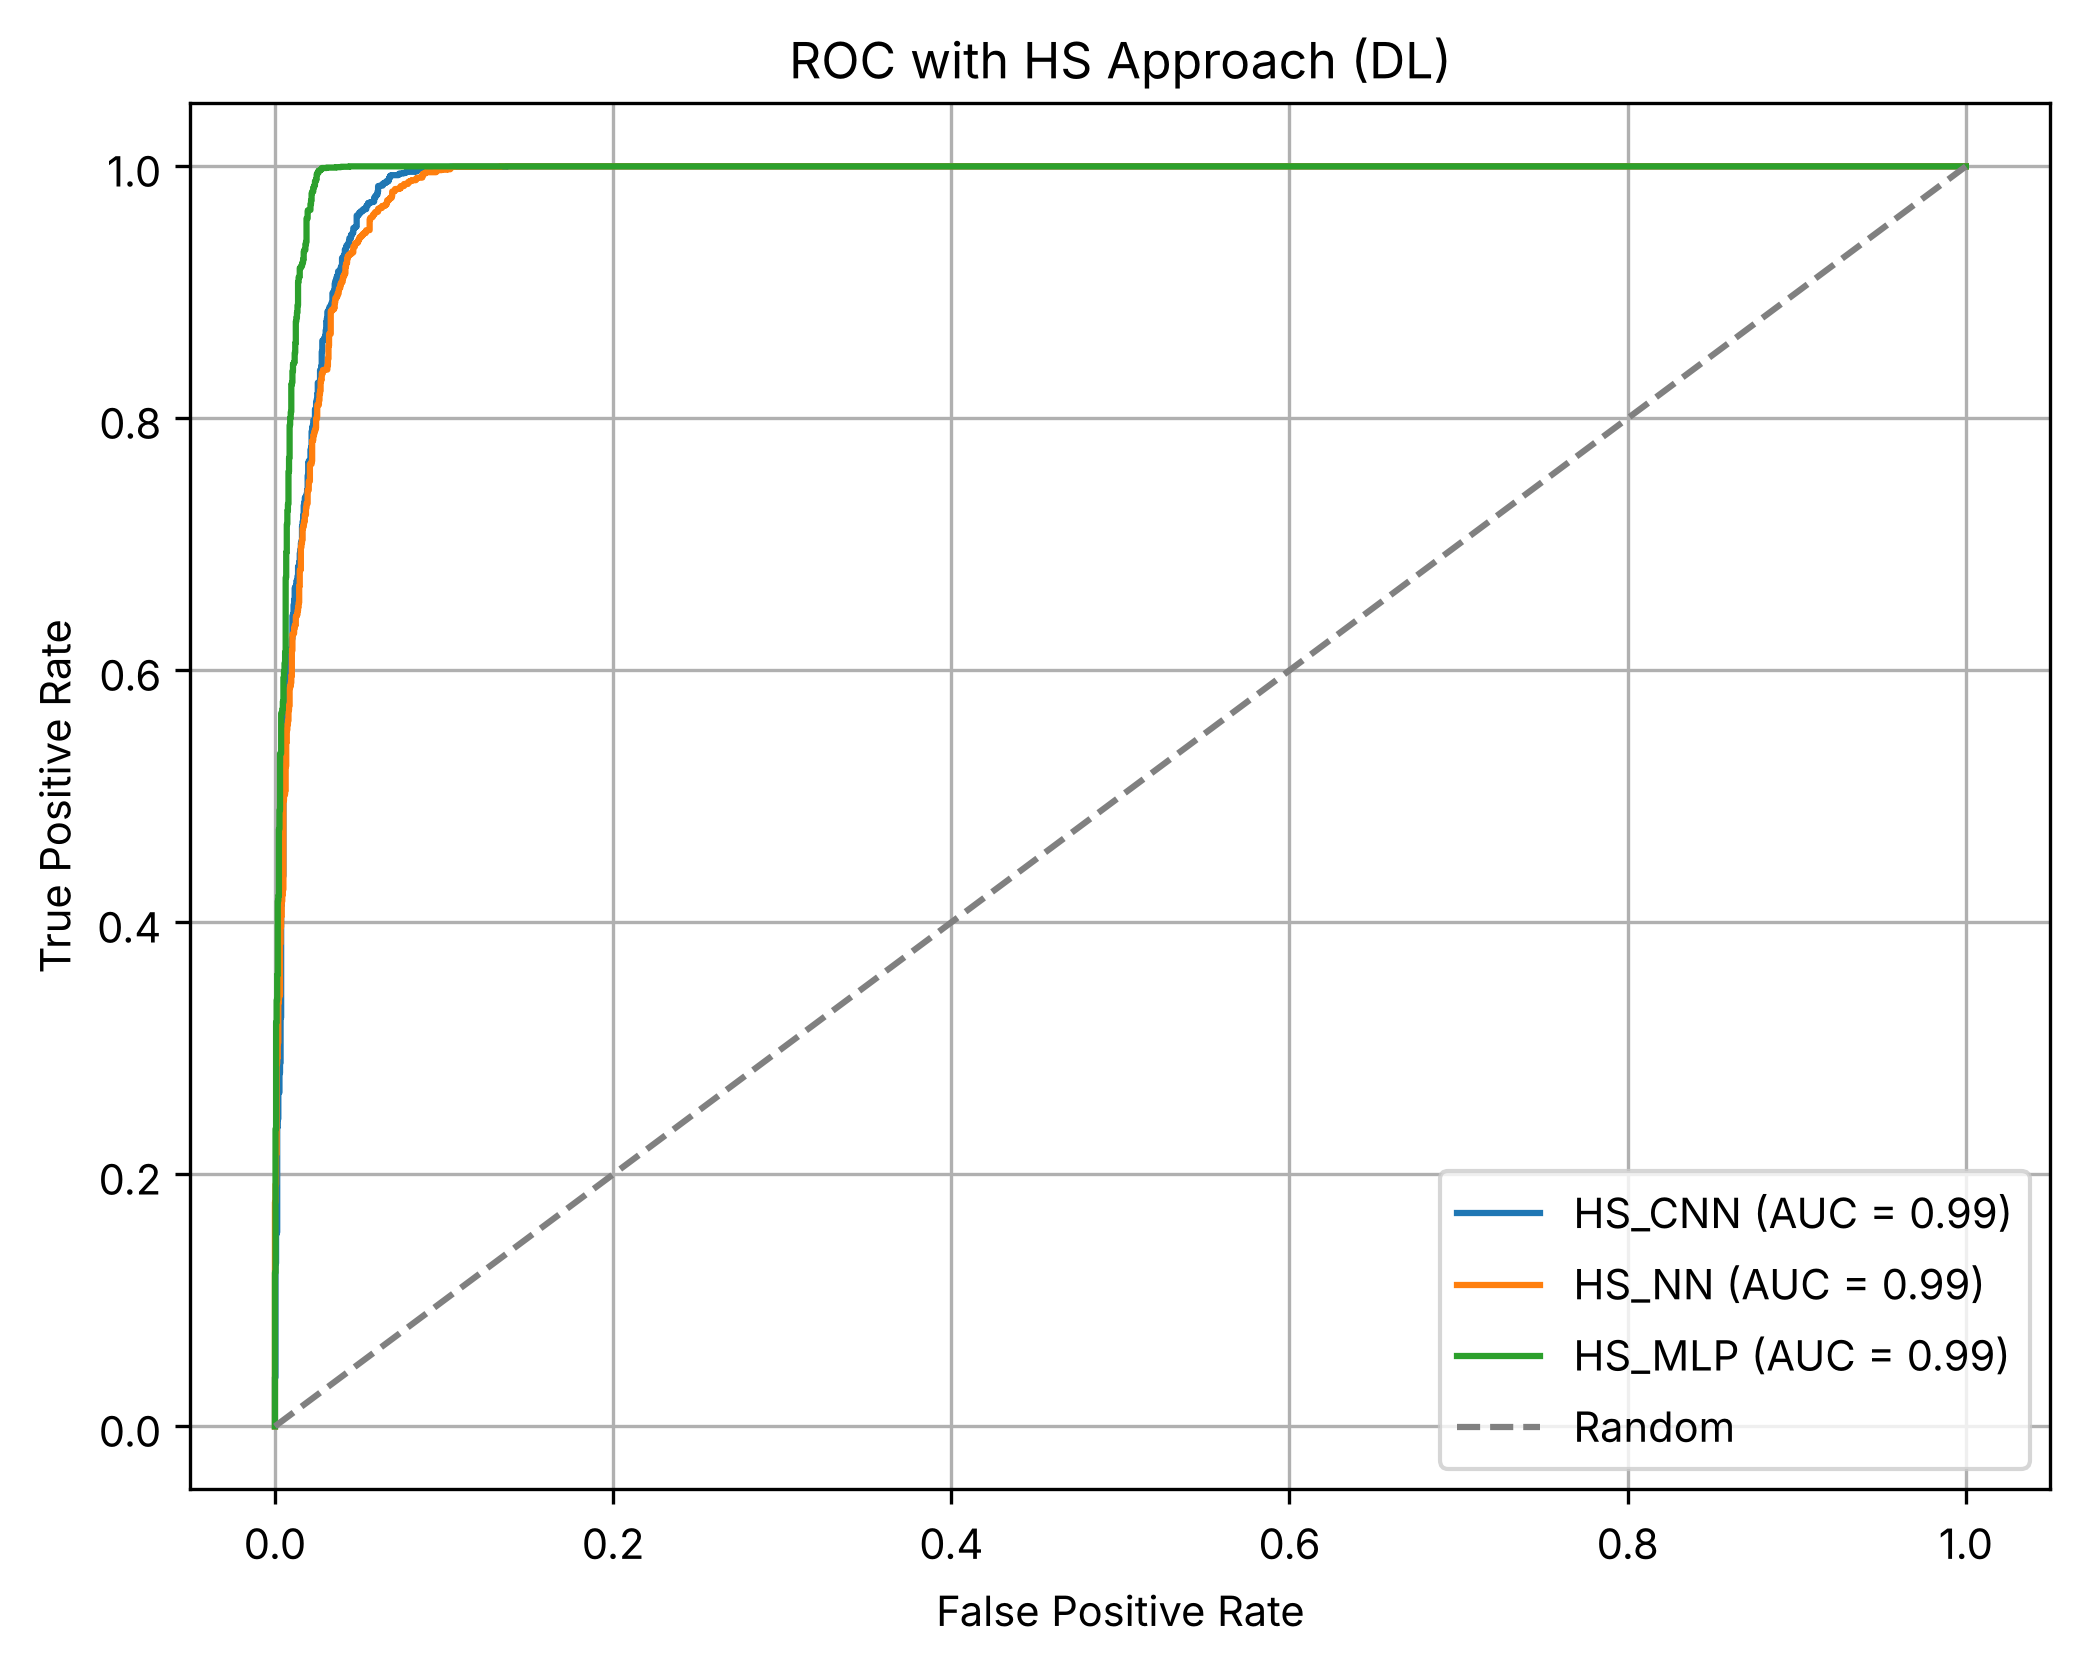
\includegraphics[width=\linewidth]{figures/roc_hs_dl.png}
  \caption{HS with DL models}
\end{subfigure}
\begin{subfigure}{0.49\linewidth}
  \centering
  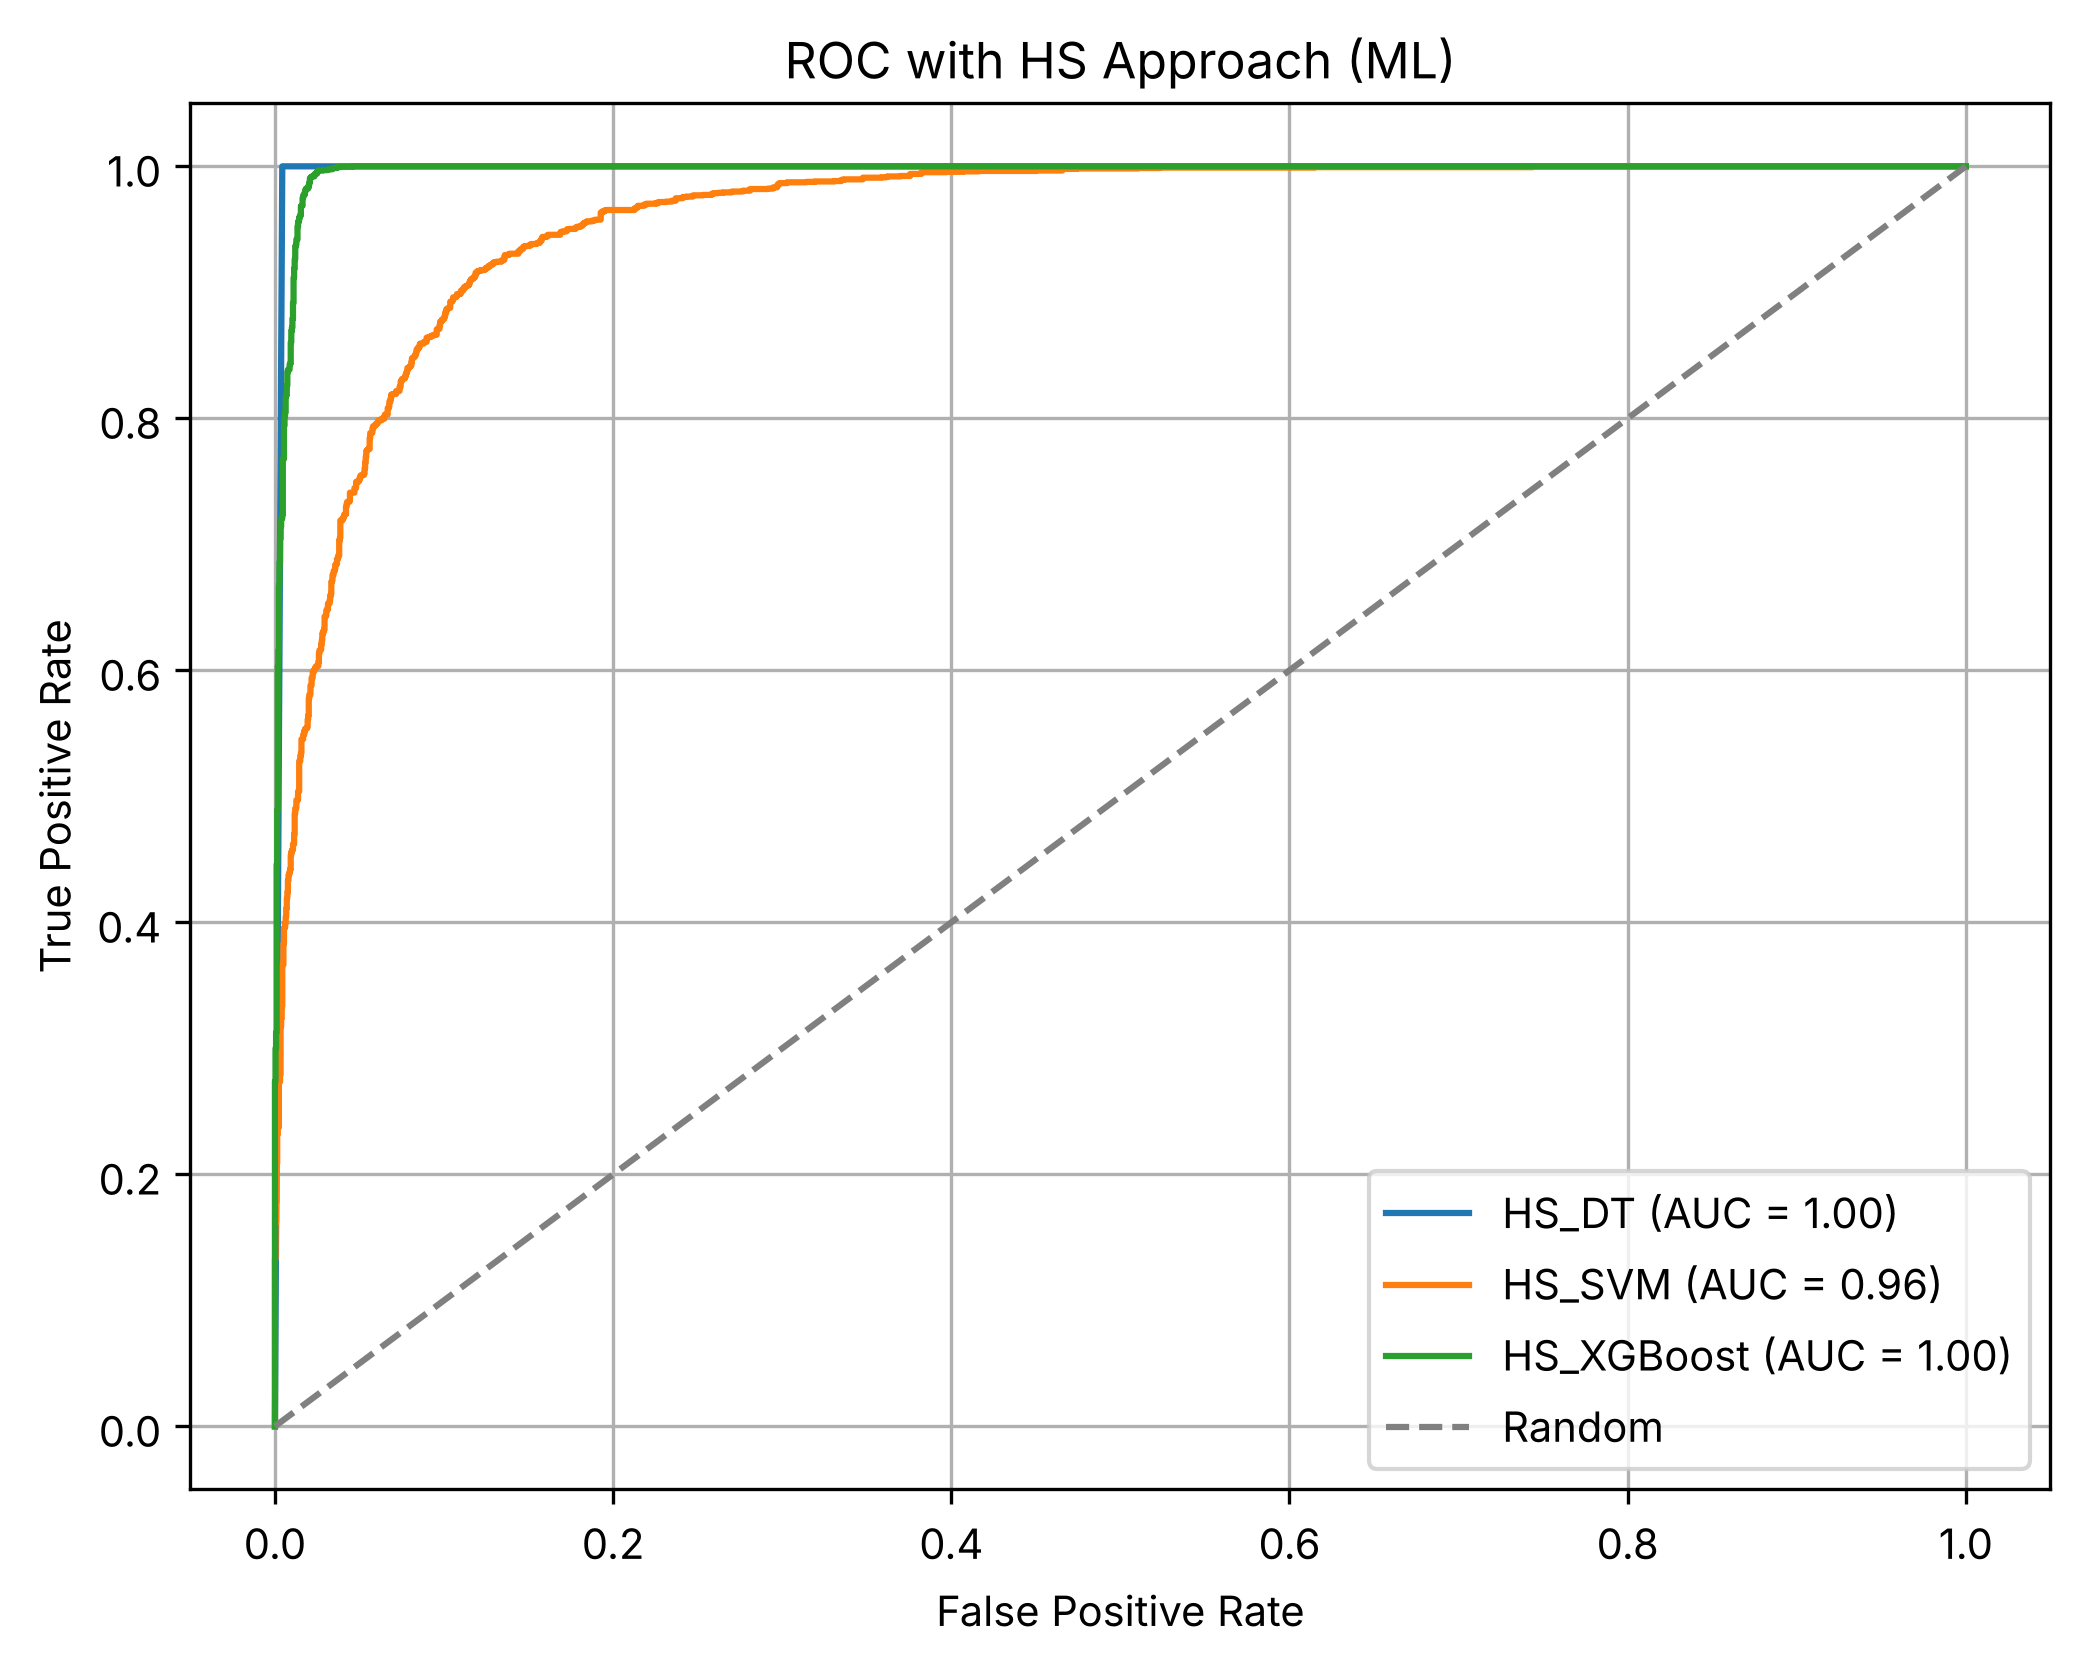
\includegraphics[width=\linewidth]{figures/roc_hs_ml.png}
  \caption{HS with ML models}
\end{subfigure}
\caption{ROC curves under Protocol A (resample before split). The
near-perfect curves are an artefact of data leakage
(Section~\ref{sec:leak}).}
\label{fig:rocA}
\end{figure}

\subsection{Data Leakage in the Resample-Before-Split Protocol}
\label{sec:leak}

Two properties of HS explain why the Protocol A results overstate how the
models would perform on new patients.

\paragraph{Duplication.} SMOTE first creates 182,347 synthetic positive
records to balance the classes. ENN then removes most of the positive
records together with 40,920 real negative records, leaving 22,239
positive and 165,144 negative records. ROS finally
duplicates each remaining positive record about 7.4 times on average to
balance the classes. When the test set is drawn from these data, its
positive records are copies of records that also occur in the training set.
Table~\ref{tab:leak} quantifies this: under Protocol A, 100\% of the
positive test records have an identical record (same features and label) in
the training set, compared with 4.6\% under Protocol B. A fully grown
decision tree can simply memorise these records, which explains its
near-perfect score.

\paragraph{Cleaning of the test population.} ENN removes every record whose
label disagrees with most of its nearest neighbours. These are exactly the
patients whose survey answers look like those of the opposite class: 19.9\%
of all real negative records are deleted before the test set is drawn. The
test set therefore no longer contains the borderline cases that make CVD
prediction from survey data hard, and the classes become artificially
separable. This is why HS raises even the smooth DL models from about
75.5\% (ROS alone, which removes no records) to 94.7--98.5\%. In a clinical
setting such patients cannot be removed.

\begin{table}[t]
\centering
\caption{Overlap between test and training sets for hybrid sampling:
percentage of test records that have an identical record (all nine features
and the label) in the training set. Negative records overlap even without
leakage because healthy respondents often give identical answers to the
nine mostly binary questions.}
\label{tab:leak}
\small
\begin{tabular}{lccc}
\toprule
Protocol & All test records & Positive (CVD) & Negative \\
\midrule
A: resample before split & 98.5\% & 100.0\% & 96.9\% \\
B: split before sampling & 40.9\% & 4.6\% & 77.1\% \\
\bottomrule
\end{tabular}
\end{table}

Both effects are well-documented forms of data
leakage~\cite{kaufman,kapoor}: information about the test data enters
model training or shapes the test data themselves. Santos et
al.~\cite{santos} showed that oversampling before cross-validation produces
over-optimistic estimates, and our results quantify the size of this bias
for CVD prediction: more than 40 percentage points of accuracy for the DT.
The cross-validation results of the original version of this study
(92.7--99.7\% accuracy for the HS models) suffer from the same problem,
because the folds were drawn from the resampled data, and are therefore
replaced by leakage-free cross-validation in Section~\ref{sec:cv}.

\subsection{Performance on Real, Unseen Records}
\label{sec:resB}

\subsubsection{The original HS pipeline under Protocol B}

Table~\ref{tab:protoB} (left) shows the same HS models trained on the
resampled training set and evaluated on 6,000 real records that were held
out before sampling. Performance drops sharply: accuracy falls to
57.4--70.8\% and the AUC to 0.57--0.81. The fully grown DT, the best model
under Protocol A, is close to chance level (AUC 0.574) because the records
it memorised do not recur among new patients. All HS models are also very
conservative on real data: their recall ranges from 18.5\% (DT) to 60.2\%
(SVM), so most CVD cases are missed. Because ENN removed the borderline
negatives from the training data, the models learn that only clear-cut
profiles are negative and place the default decision threshold of 0.5 far
from where it would be on the real population.

\begin{table}[t]
\centering
\caption{Test performance under Protocol B (6,000 real records, 3,000 per
class, held out before any sampling). Left: original HS pipeline (nine
features, hybrid sampling of the training data, threshold 0.5). Right:
improved pipeline (all 21 features, class weights, regularised models,
threshold tuned on the validation set). All values in \%.}
\label{tab:protoB}
\footnotesize
\setlength{\tabcolsep}{3.5pt}
\begin{tabular}{l|ccccc|ccccc}
\toprule
 & \multicolumn{5}{c|}{Original HS pipeline} & \multicolumn{5}{c}{Improved pipeline} \\
Model & Acc. & Prec. & Rec. & F1 & AUC & Acc. & Prec. & Rec. & F1 & AUC \\
\midrule
\inputrows{tables/protocol_b_test.tex}
\bottomrule
\end{tabular}
\end{table}

\subsubsection{Ablation study}

To identify which design choices limit performance on real data, we varied
them one at a time for XGBoost and the DT (Table~\ref{tab:ablation}). The
AUC measures how well a model ranks patients by risk, independently of the
threshold; accuracy is reported both at the default threshold of 0.5 and at
the threshold tuned on the validation set.

\begin{table}[t]
\centering
\caption{Ablation study under Protocol B (real test set). ``Tuned'' denotes
the threshold that maximises Youden's $J$ on the validation set.}
\label{tab:ablation}
\small
\begin{tabular}{llccc}
\toprule
Model & Configuration & AUC (\%) & Acc.\ @ 0.5 (\%) & Acc.\ @ tuned (\%) \\
\midrule
XGBoost & 9 features, HS (original) & 74.31 & 61.58 & 68.28 \\
XGBoost & 9 features, ROS only & 82.06 & 74.35 & 74.25 \\
XGBoost & 9 features, no resampling & 82.25 & 53.27 & 74.55 \\
XGBoost & 21 features, no resampling & 83.54 & 54.75 & 75.25 \\
XGBoost & 21 features, class weights, regularised (improved) & 83.99 & -- & 76.00 \\
\midrule
DT & 9 features, HS, full depth (original) & 57.40 & 57.40 & 57.40 \\
DT & 21 features, class weights, depth 8 (improved) & 82.50 & -- & 74.90 \\
\bottomrule
\end{tabular}
\end{table}

Four findings emerge. First, hybrid sampling is the main cause of the loss:
replacing it with ROS alone raises the AUC of XGBoost from 0.743 to 0.821,
and dropping resampling altogether gives the same AUC (0.823), showing that
synthetic records and ENN cleaning distort the data rather than add
information. Second, without resampling the default threshold of 0.5 is
unsuitable for imbalanced data (53.3\% accuracy, because almost every
record is predicted negative), whereas a threshold tuned on the validation
set restores 74.6\% accuracy; resampling and threshold tuning address the
same problem, but tuning does so without altering the data. Third, using all
21 features instead of the nine correlation-selected ones increases the AUC
from 0.823 to 0.835: features such as sex, income, BMI and education carry
predictive information that a univariate correlation ranking misses.
Fourth, regularisation (shallow, early-stopped boosting and a depth-limited
tree) prevents the models from memorising individual records; it turns the
DT from a near-random classifier into a competitive model (AUC 0.825).

\subsubsection{The improved pipeline}

Table~\ref{tab:protoB} (right) shows that the improved pipeline raises
every model on real, unseen records, and Fig.~\ref{fig:improved}
summarises its results. Accuracy
increases to 74.9--76.0\%, recall to 78.8--82.8\% and the AUC to
0.825--0.840. The largest gains concern recall: the improved XGBoost
detects 82.8\% of CVD cases, compared with 30.5\% for the original HS
XGBoost, and the improved DT detects 78.9\% compared with 18.5\%. The ROC
curves of all improved models nearly coincide (Fig.~\ref{fig:rocB}), and
logistic regression performs on par with XGBoost and the three DL models.
The confusion matrices (Fig.~\ref{fig:cmB}) show a balanced error profile:
the improved XGBoost correctly identifies 2,483 of 3,000 CVD cases and
2,077 of 3,000 non-CVD cases. The learning curves of the DL models
(Fig.~\ref{fig:lcB}) show the validation loss decreasing for about ten
epochs and then levelling off; training stops three epochs after the last
improvement and the best weights are restored, which prevents
over-fitting. The training loss is computed with class weights and is
therefore not directly comparable to the unweighted validation loss.

\begin{figure}[t]
\centering
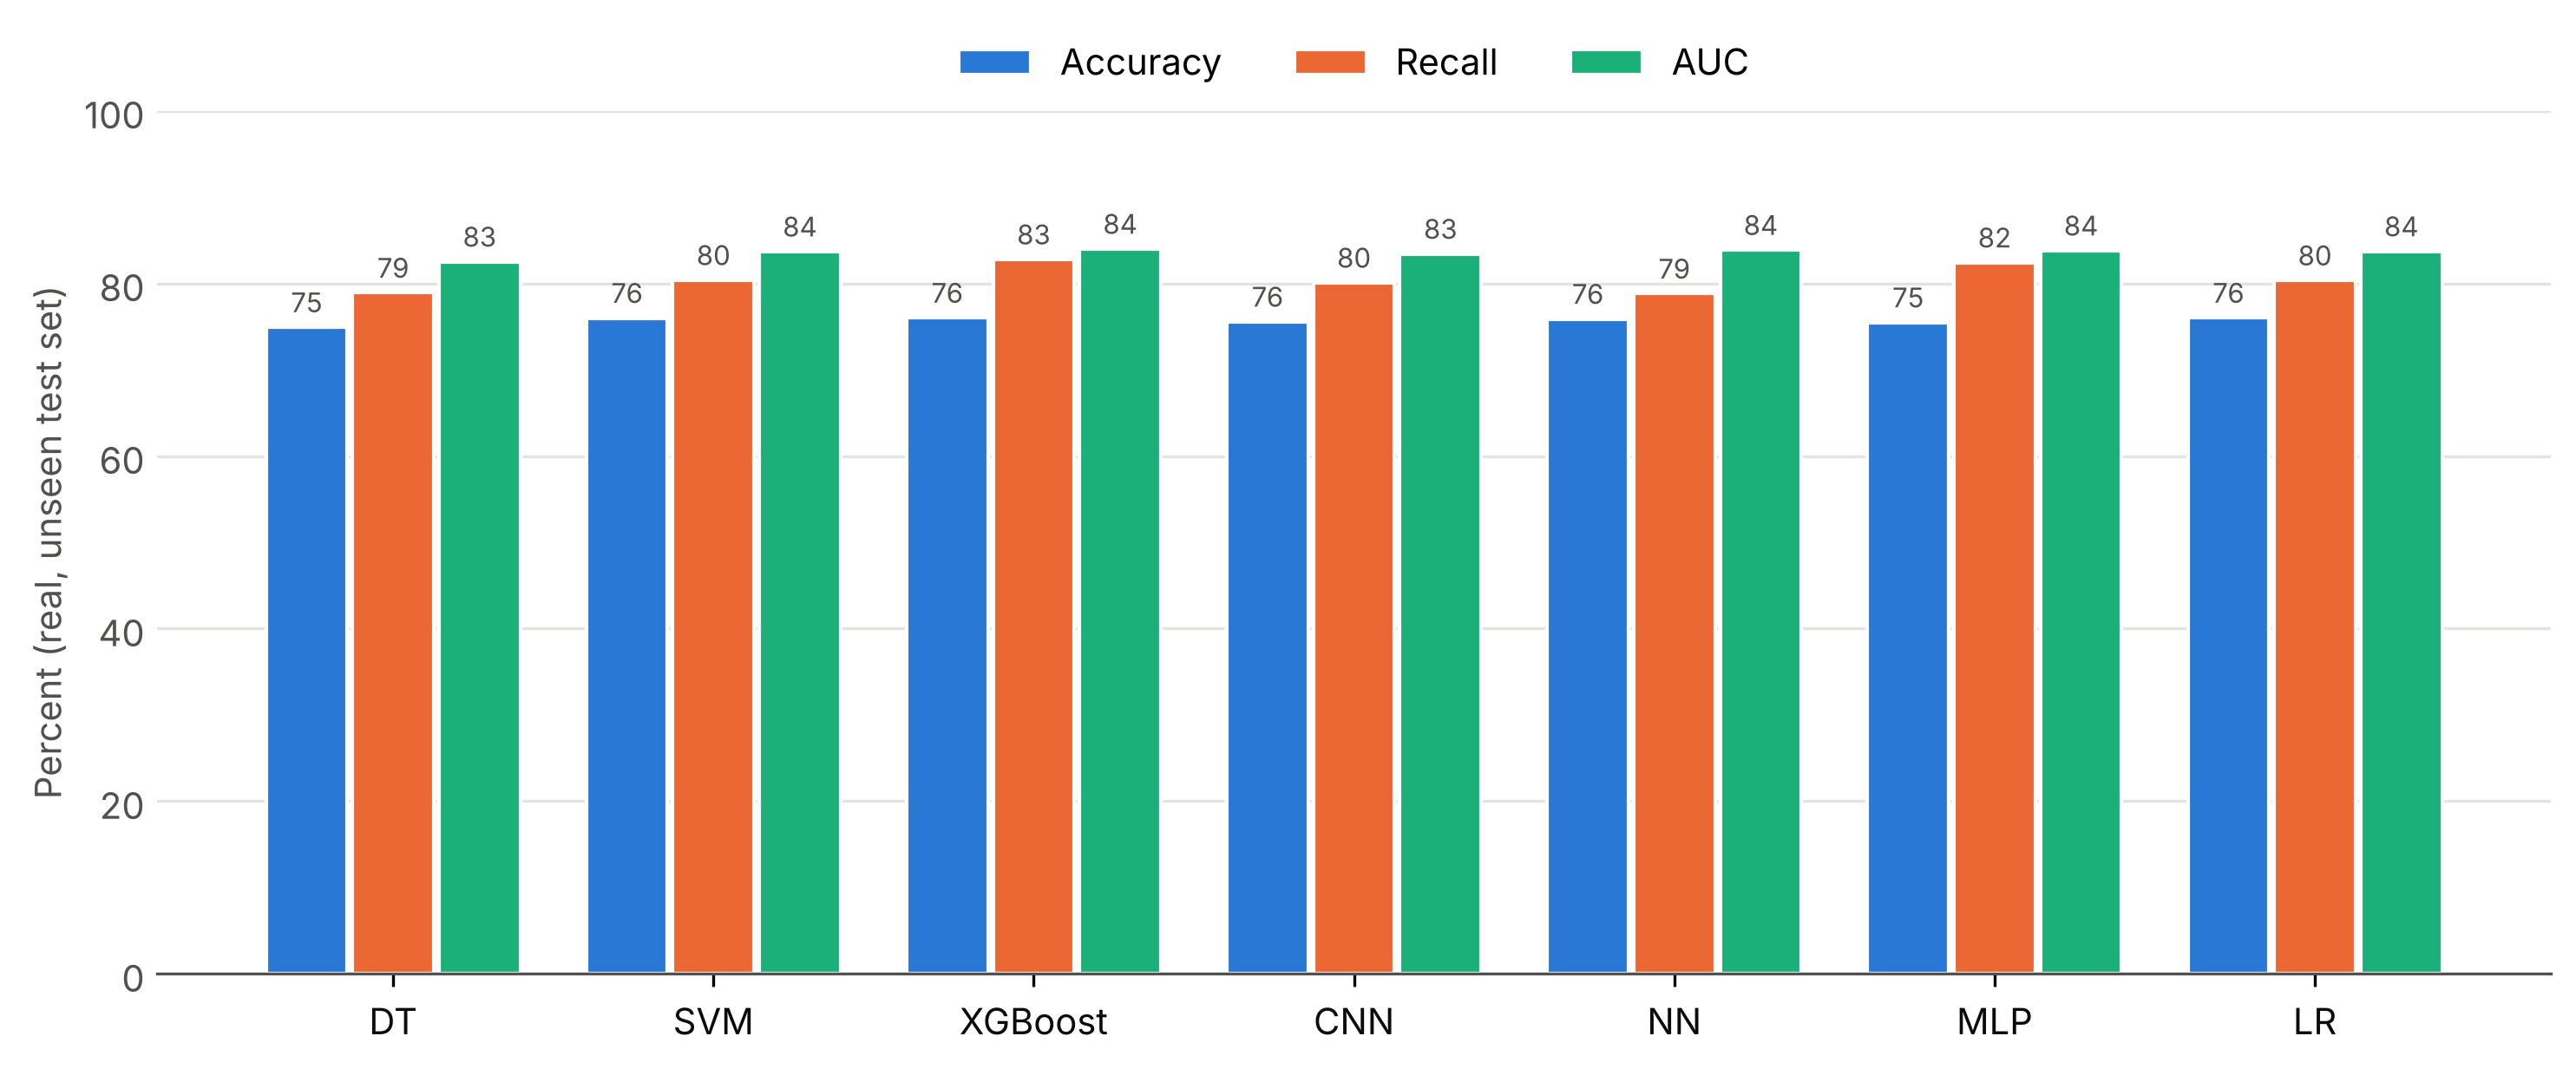
\includegraphics[width=0.9\linewidth]{figures/improved_results.png}
\caption{Accuracy, recall and AUC of the improved models on the real,
unseen test set (Protocol B).}
\label{fig:improved}
\end{figure}

\begin{figure}[t]
\centering
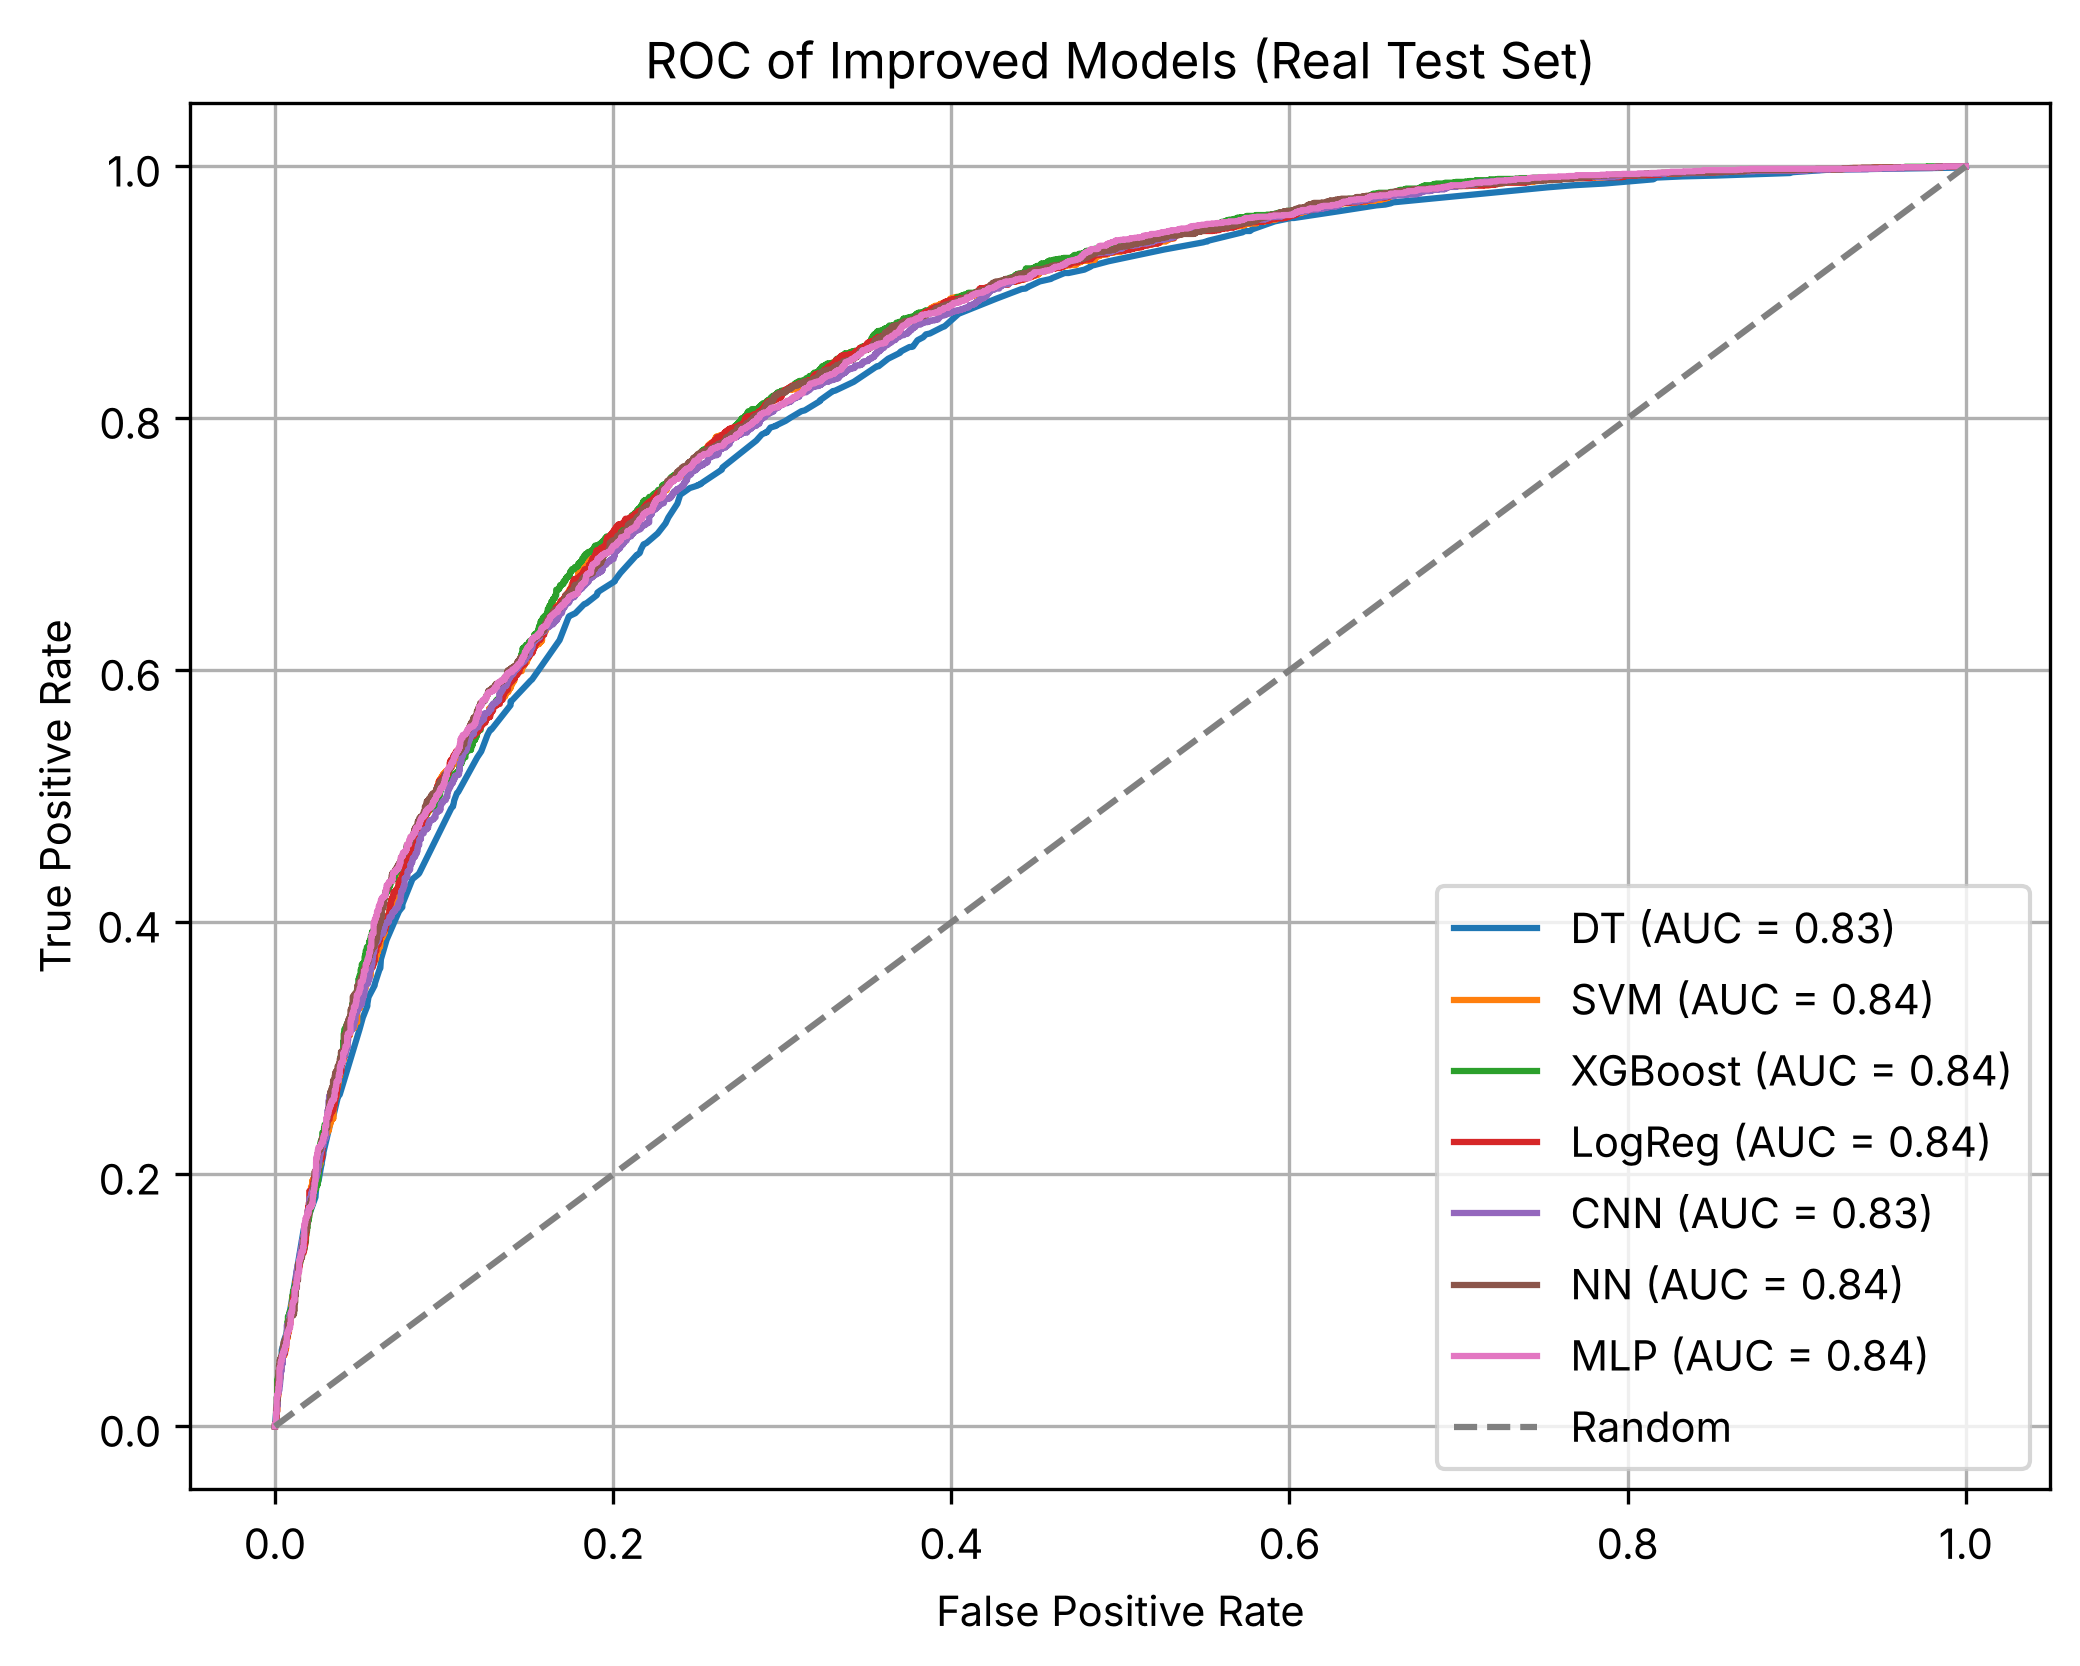
\includegraphics[width=0.6\linewidth]{figures/roc_improved.png}
\caption{ROC curves of the improved models on the real, unseen test set
(Protocol B).}
\label{fig:rocB}
\end{figure}

\begin{figure}[t]
\centering
\begin{subfigure}{0.32\linewidth}
  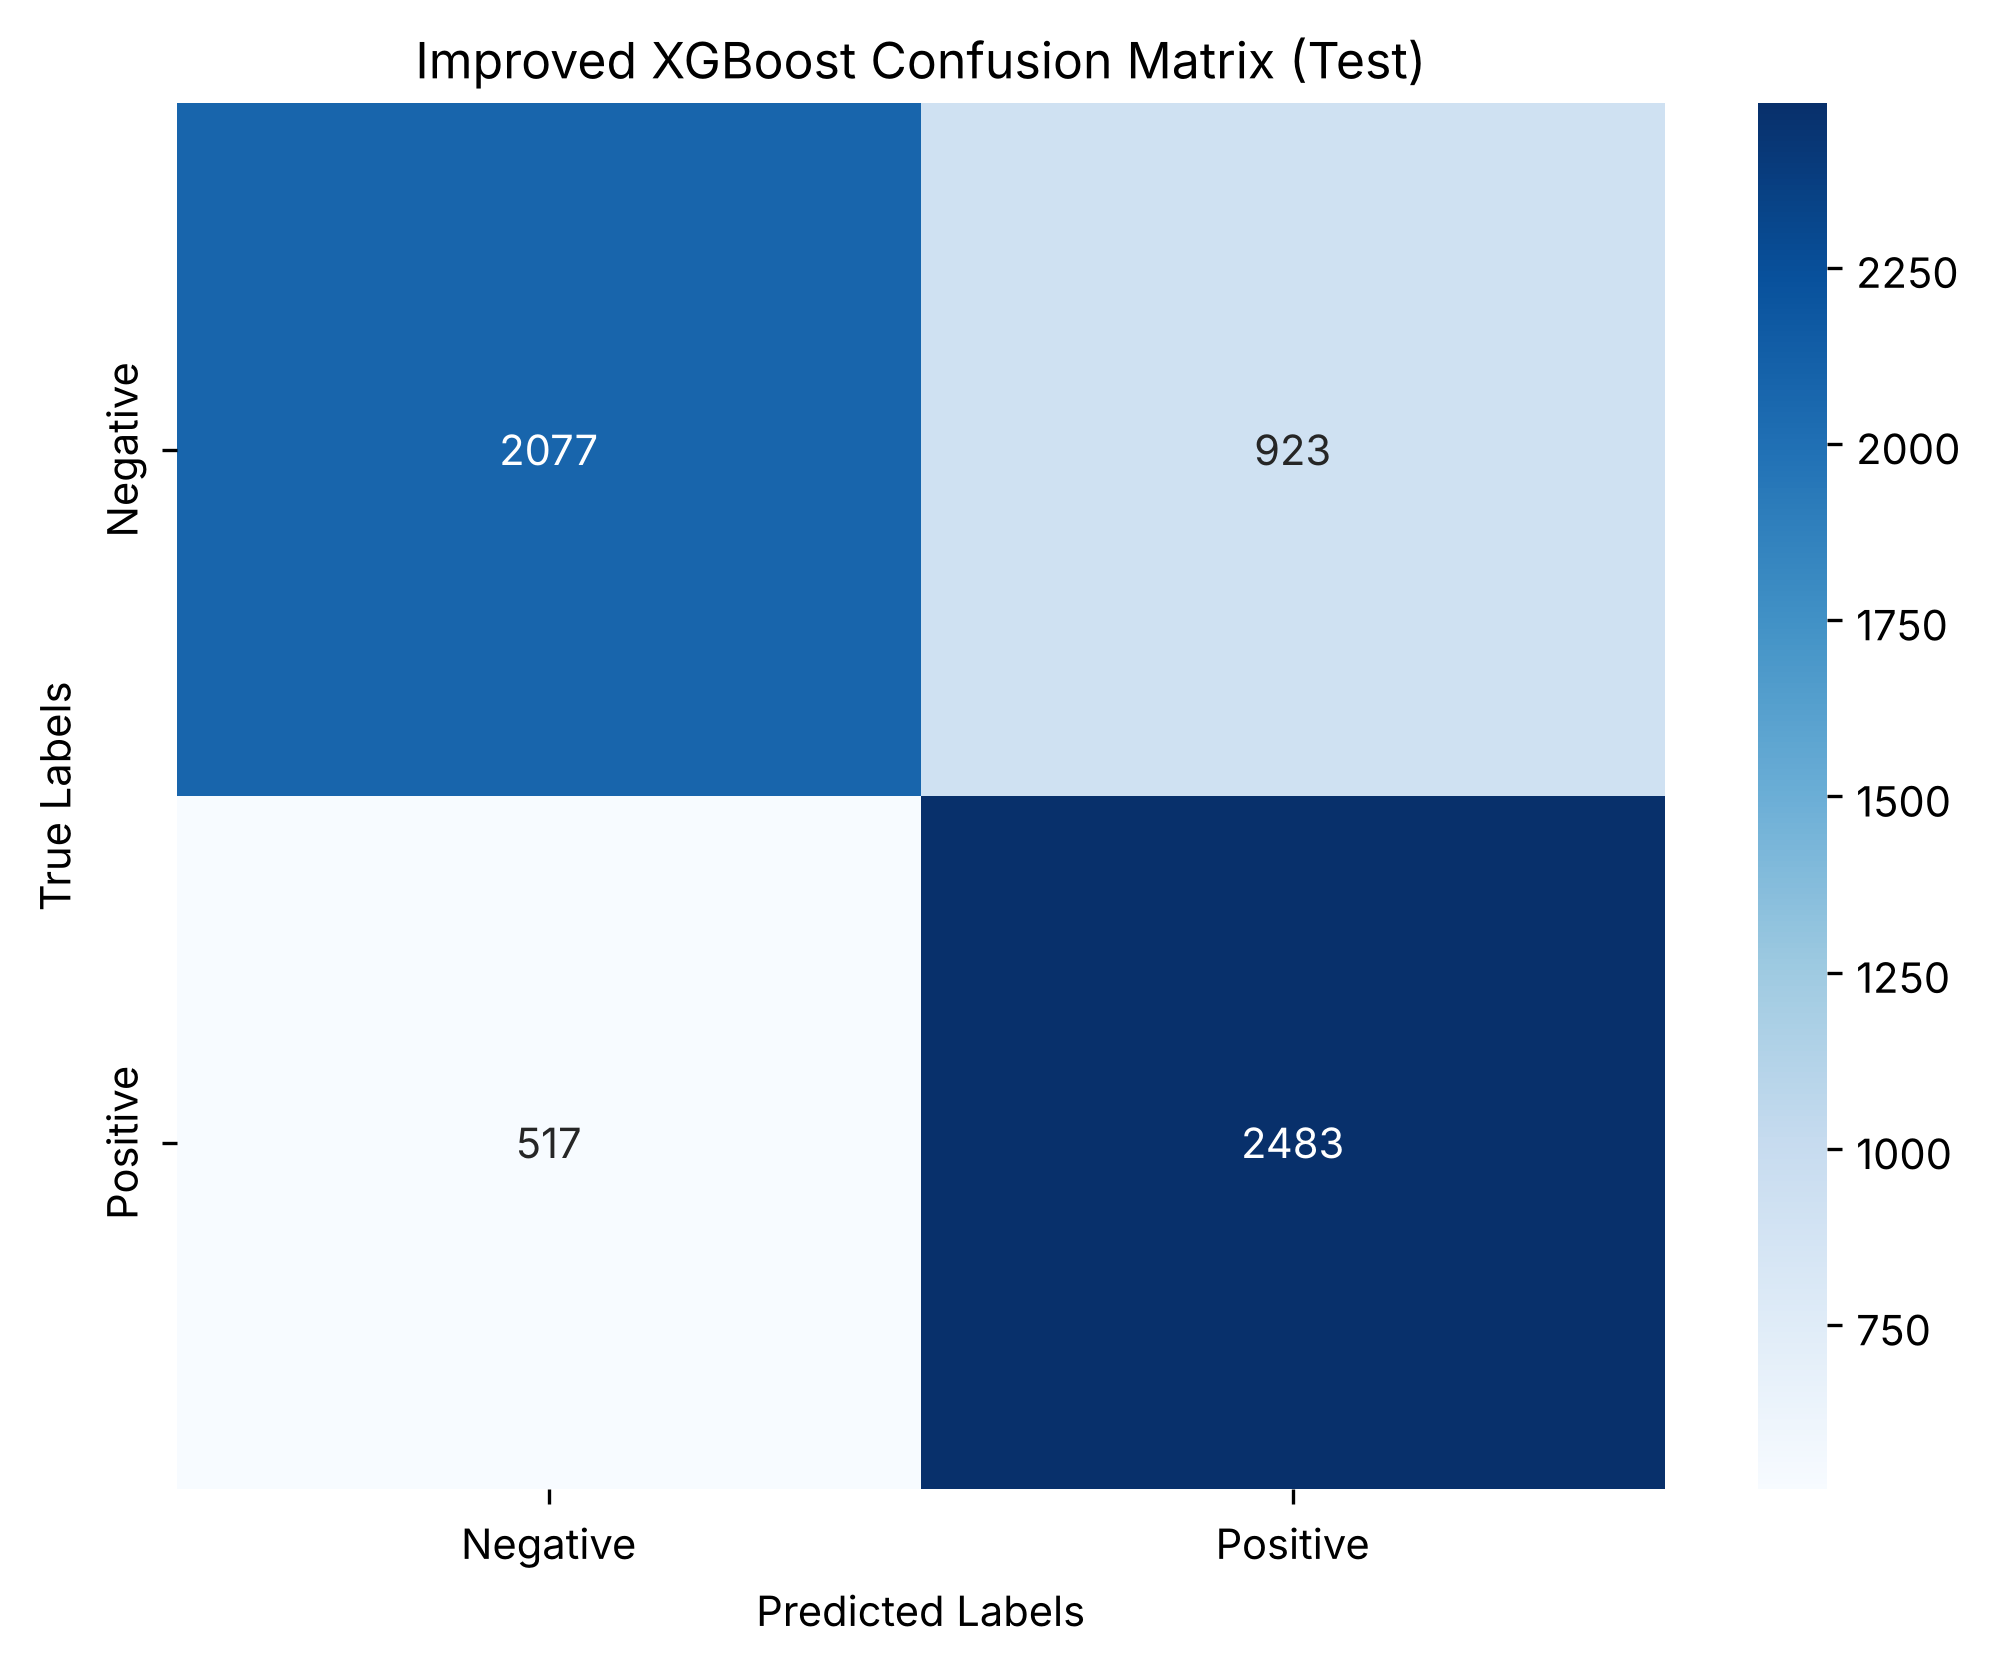
\includegraphics[width=\linewidth]{figures/improved_confusion_matrix_XGBoost.png}
  \caption{XGBoost}
\end{subfigure}
\begin{subfigure}{0.32\linewidth}
  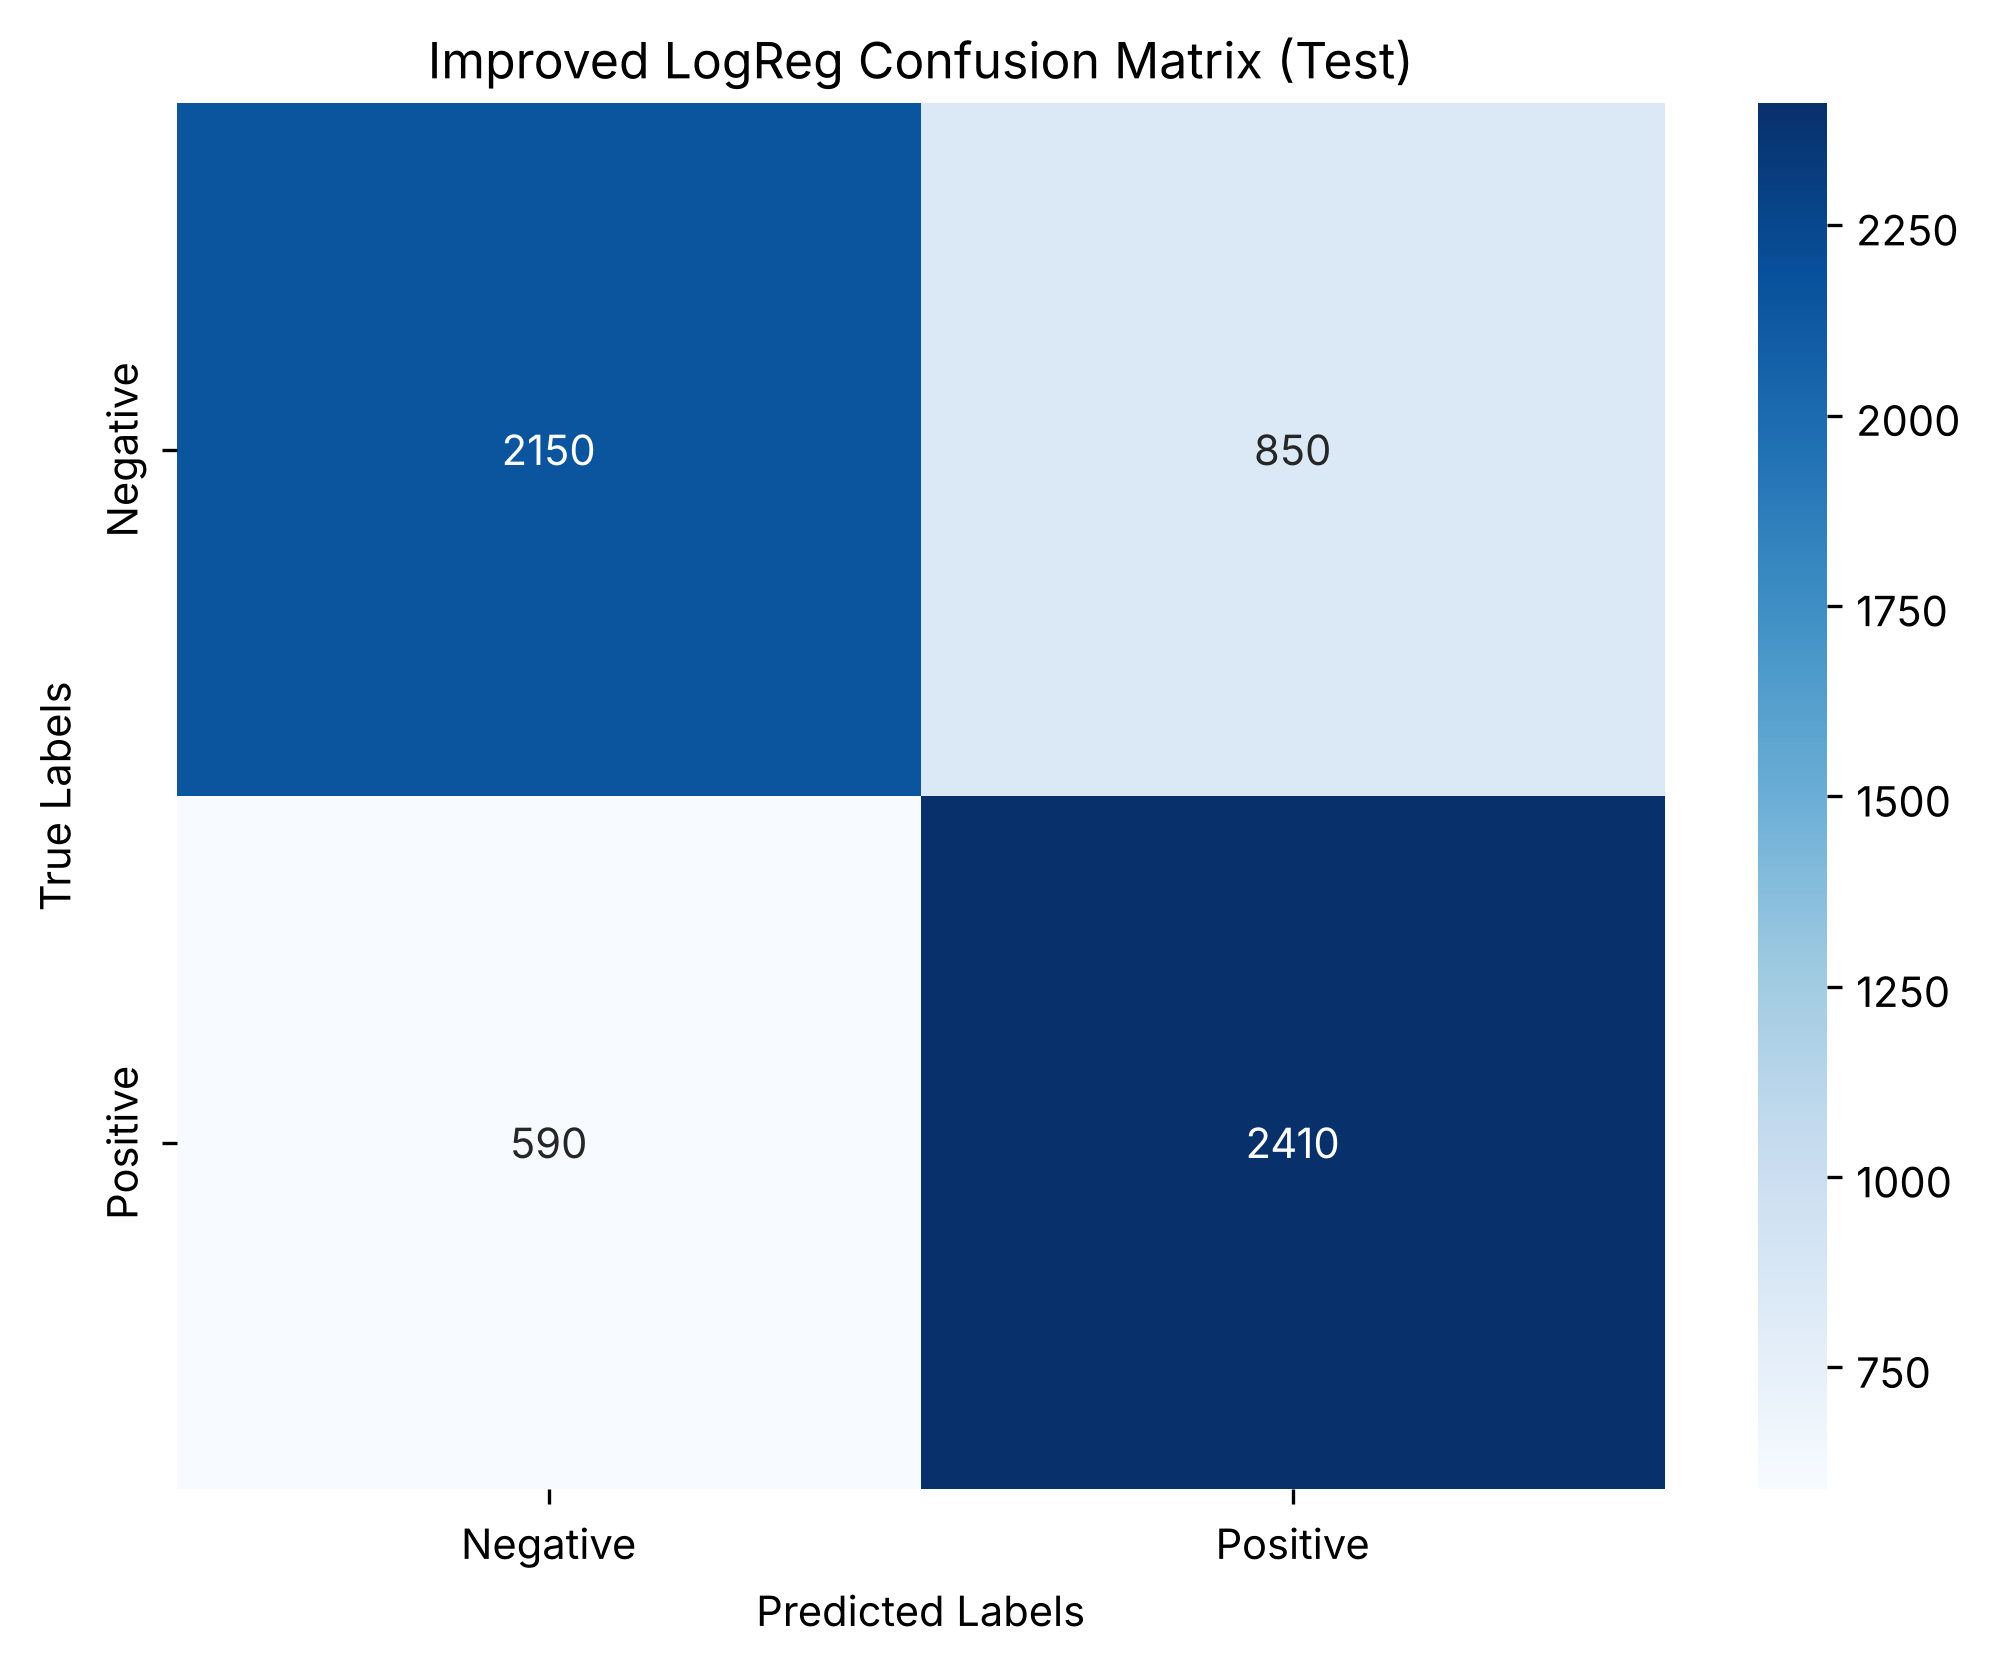
\includegraphics[width=\linewidth]{figures/improved_confusion_matrix_LogReg.png}
  \caption{Logistic regression}
\end{subfigure}
\begin{subfigure}{0.32\linewidth}
  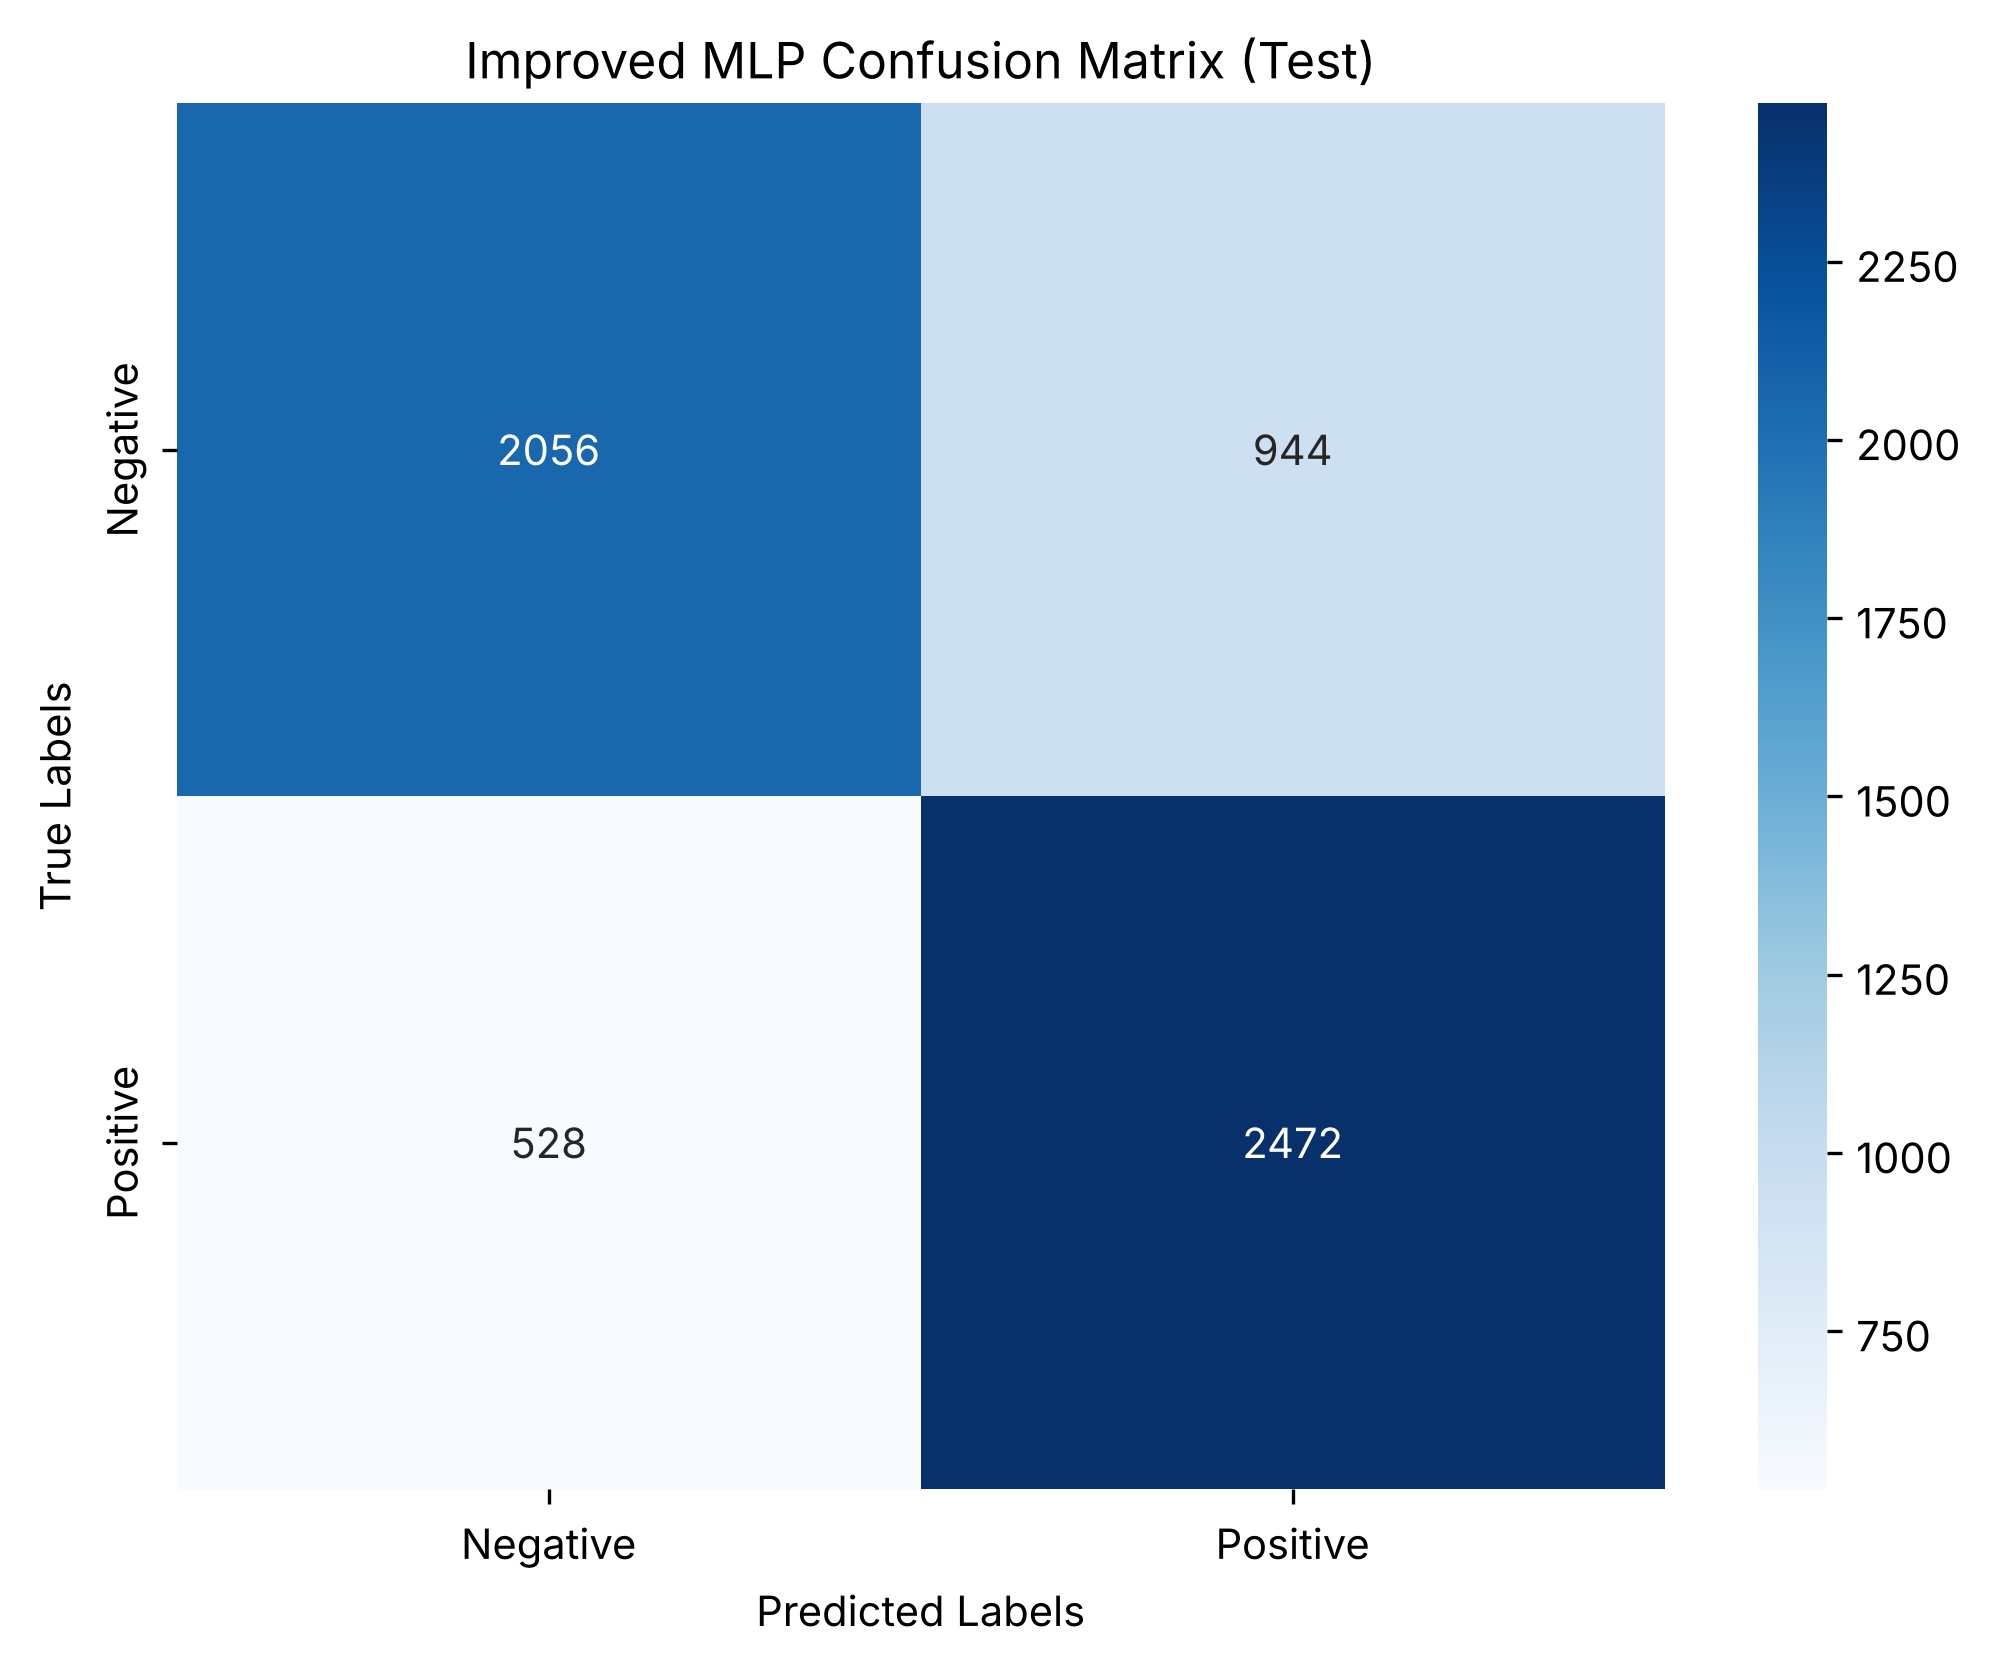
\includegraphics[width=\linewidth]{figures/improved_confusion_matrix_MLP.png}
  \caption{MLP}
\end{subfigure}
\caption{Confusion matrices of improved models on the real test set
(Protocol B, 3,000 records per class).}
\label{fig:cmB}
\end{figure}

\begin{figure}[t]
\centering
\begin{subfigure}{\linewidth}
  \centering
  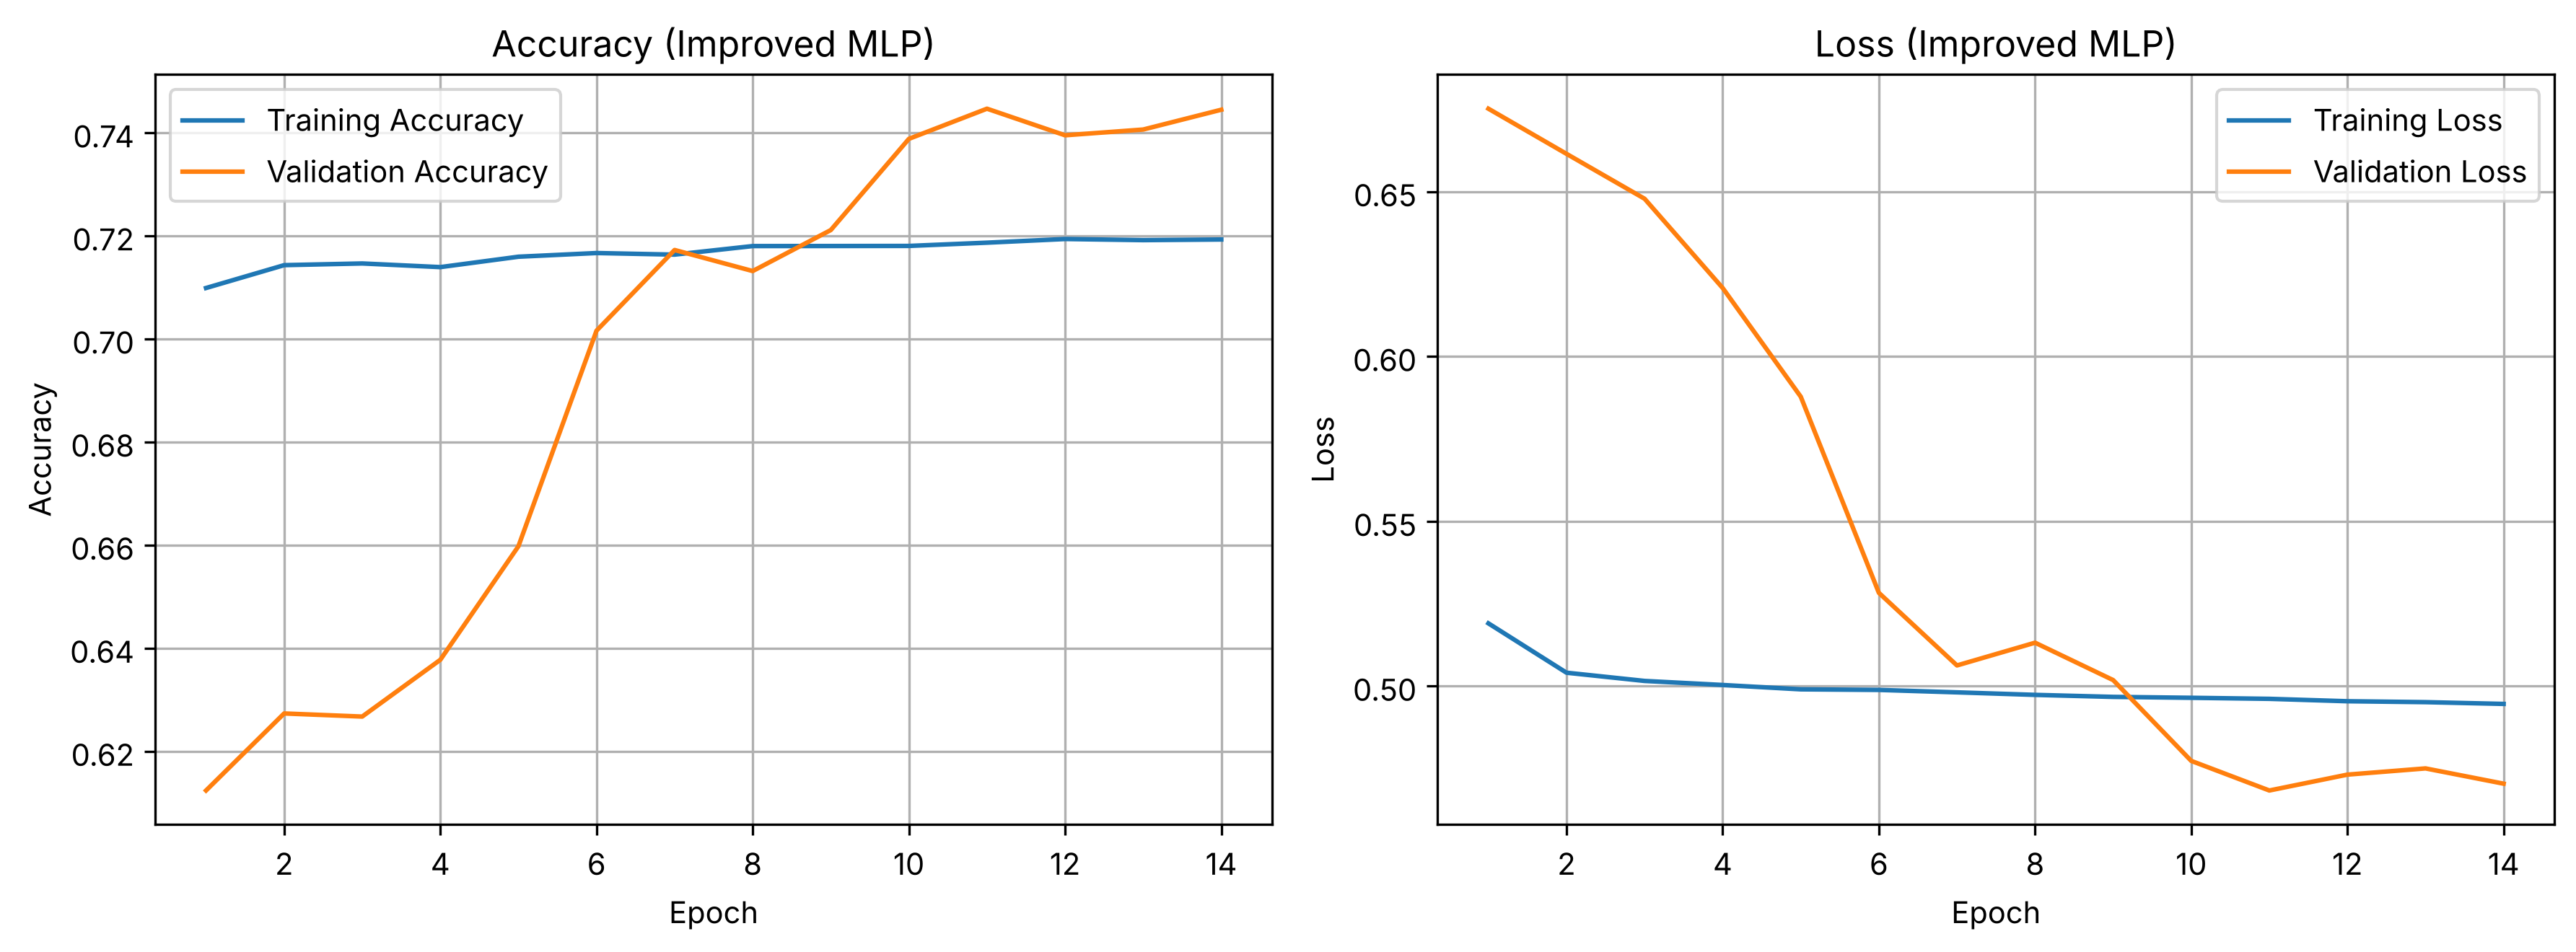
\includegraphics[width=0.85\linewidth]{figures/improved_learning_curve_MLP.png}
  \caption{MLP}
\end{subfigure}
\begin{subfigure}{\linewidth}
  \centering
  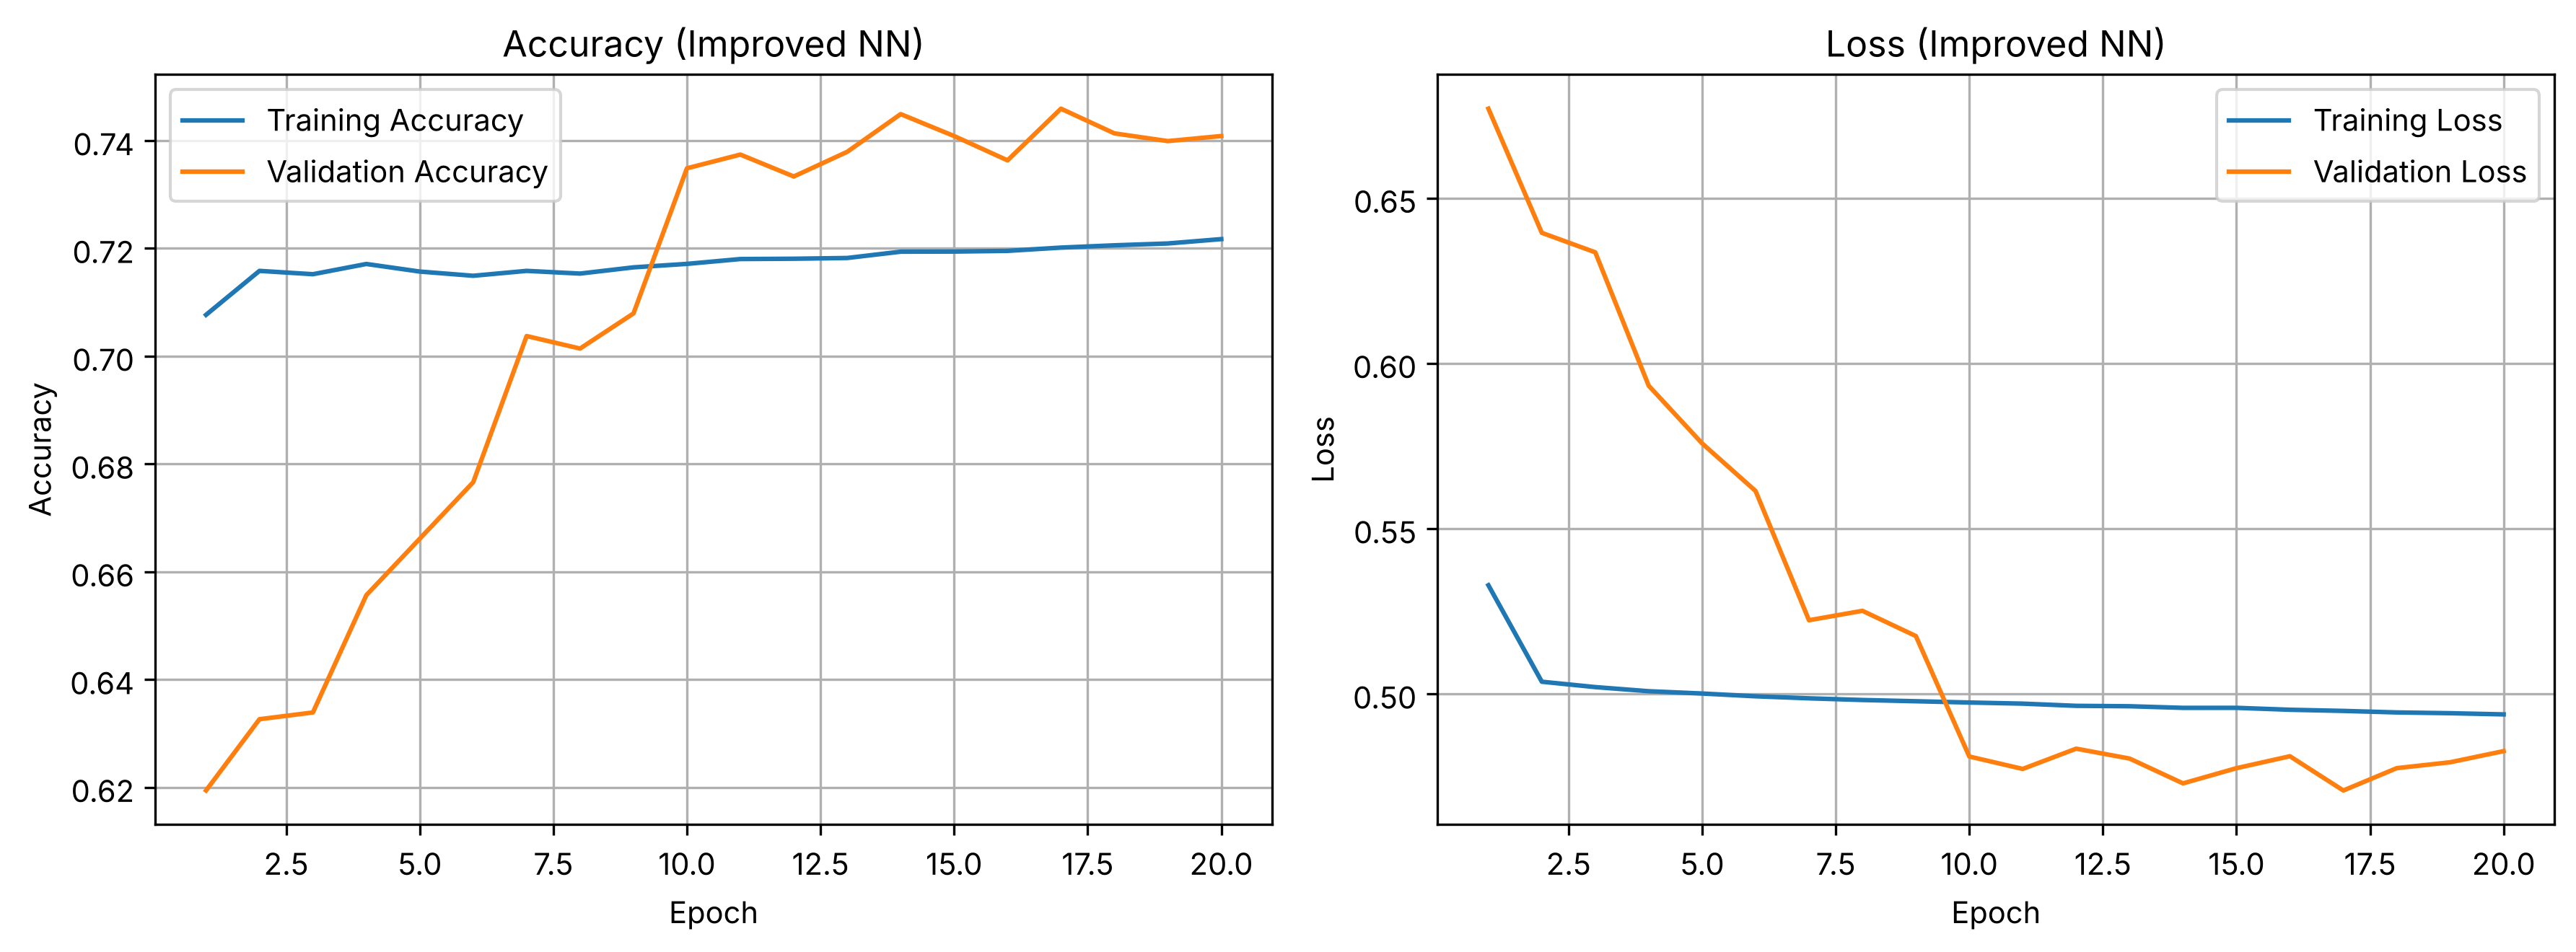
\includegraphics[width=0.85\linewidth]{figures/improved_learning_curve_NN.png}
  \caption{NN}
\end{subfigure}
\caption{Training and validation accuracy and loss of the improved DL
models; training stops early once the validation loss no longer
improves.}
\label{fig:lcB}
\end{figure}

\subsubsection{Five-fold cross-validation}
\label{sec:cv}

To check that these results do not depend on one particular split, the
improved models were evaluated with stratified five-fold cross-validation
on the 223,781 real records that are not in the test set. In every fold,
20\% of the training portion was set aside for early stopping and threshold
tuning, and the held-out fold kept the real prevalence of about 10.3\%.
Table~\ref{tab:cv} reports the mean and standard deviation over the folds.
The AUC (0.824--0.839) and recall (78.9--82.5\%) agree with the test-set
results and vary little between folds (standard deviation of the AUC at
most 0.64 percentage points), confirming that the estimates are stable.
Accuracy (70.8--72.2\%) is lower than on the balanced test set because the
tuned threshold trades specificity for sensitivity and negatives make up
almost 90\% of each fold.

\begin{table}[t]
\centering
\caption{Five-fold cross-validation of the improved models on real records
at the natural prevalence of CVD (about 10.3\%); mean $\pm$ standard
deviation over the folds, in \%.}
\label{tab:cv}
\small
\begin{tabular}{lccccc}
\toprule
Model & Accuracy & Precision & Recall & F1 Score & AUC \\
\midrule
\inputrows{tables/cv_improved.tex}
\bottomrule
\end{tabular}
\end{table}

Precision and F1 are much lower in cross-validation than on the balanced
test set because the folds keep the real prevalence. At a prevalence of
10\%, even a model with about 80\% sensitivity and 70\% specificity flags
roughly three to four healthy respondents for every true CVD case
(precision about 22\%). This is an inherent property of screening for a
condition of low prevalence, not a defect of a particular model, and it
should guide how such models are used: as inexpensive pre-screening tools
that refer at-risk individuals for clinical assessment, not as diagnostic
tests.

\subsection{Comparison with Existing Studies}
\label{sec:compare}

Table~\ref{tab:literature} compares the proposed method with existing
studies. With a few exceptions, previous studies achieved accuracy rates
between 82\% and 96\%, and studies on small datasets such as the Cleveland
heart disease data (303 records) report the highest values. These figures
are not directly comparable: the studies use different datasets with
different clinical variables, and several do not state whether resampling
or feature selection was performed before the data were split. Our results
show that this choice alone can change the reported accuracy of the same
model on the same data from 57\% to 99.8\%. For the proposed method we
therefore report the leakage-free results on 6,000 real BRFSS records. Of
the studies listed, Amarbayasgalan et al.~\cite{amarbayasgalan} used the
KNHANES survey (25,340 records), which is closest in nature to BRFSS.

\begin{table}[t]
\centering
\caption{Comparison of the proposed method with existing studies. The
proposed results are leakage-free (Protocol B, real held-out test set).}
\label{tab:literature}
\footnotesize
\setlength{\tabcolsep}{3pt}
\begin{tabular}{lllccccc}
\toprule
Study & Dataset & Method & Acc. (\%) & Prec. (\%) & Rec. (\%) & F1 (\%) & AUC (\%) \\
\midrule
M. Bhatt et al.~\cite{bhatt} & CVD dataset & XGBoost & 87.02 & 89.62 & 82.11 & 86.30 & 95.00 \\
S. K. Mohan et al.~\cite{mohan} & Cleveland & Hybrid (HRFLM) & 88.40 & 90.10 & 92.80 & 90.00 & -- \\
N. L. Fitriyani et al.~\cite{fitriyani} & Cleveland & SMOTEENN + XGBoost & 95.90 & 97.14 & 94.67 & 95.35 & -- \\
W. Chang et al.~\cite{chang} & Beijing dataset & Hybrid XGBSVM & 91.70 & -- & -- & -- & 93.90 \\
A. A. Almazroi et al.~\cite{almazroi} & Cleveland & DNN & 82.49 & -- & 87.24 & 84.41 & -- \\
J. P. Li et al.~\cite{li} & Cleveland & SVM (Linear) & 85.00 & -- & 75.00 & -- & -- \\
T. Amarbayasgalan et al.~\cite{amarbayasgalan} & KNHANES & Two DNNs & 89.20 & 91.10 & 92.00 & 91.50 & 97.54 \\
\midrule
Proposed (improved) & BRFSS & XGBoost & 76.00 & 72.90 & 82.77 & 77.52 & 83.99 \\
Proposed (improved) & BRFSS & Logistic regression & 76.00 & 73.93 & 80.33 & 77.00 & 83.70 \\
Proposed (improved) & BRFSS & MLP & 75.47 & 72.37 & 82.40 & 77.06 & 83.79 \\
\bottomrule
\end{tabular}
\end{table}

\subsection{Limitations}

The BRFSS data are self-reported and cross-sectional: the target records a
past diagnosis of coronary heart disease or myocardial infarction, so the
models identify individuals who resemble patients with a history of CVD
rather than predict future events. Self-reported survey answers also carry
less information than clinical measurements, which limits the attainable
discrimination. The models were developed and tested on a single survey
year without external validation, and the calibration of the predicted
probabilities was not assessed. The balanced test set makes accuracy
comparable across protocols, but precision and F1 depend on prevalence, and
the cross-validation results indicate the values to expect in a general
population.
